\section{Mikroprozessoren}\label{2}

Für das Verständnis eines DSPs ist das Verständnis der zu Grunde liegenden Hardware unumgänglich. Hierzu wird zunächst in Kapitel \ref{2.1} der Begriff 'Echtzeit' erklärt. In der praktischen Anwendung ist die Signalverarbeitung ein Echtzeit-Problem, weswegen dieser Begriff eine wichtige Grundlage bildet. Des weiteren führt dieses Kapitel noch andere ebenfalls wichtige Begriffe ein, beispielsweise 'harte Echtzeit' oder auch 'Deadlines'.\\
Kapitel \ref{2.2} befasst sich mit der Bauweise von Speicherelementen. Dazu zählen 'Random-Access-Memory' (RAM), 'Read-Only-Memory' (ROM), 'Flash'-Speicher (EEPROM) sowie Caches. Insbesondere wird auf Vor- und Nachteile dieser Optionen eingegangen.\\
Bestandteile des Kapitels \ref{2.3} sind verschiedene Architekturen, wobei Harvard sowie Von-Neumann eine tragende Rolle spielen.
Im Folgenden befasst sich Kapitel \ref{2.4} mit weitergehender Architektur, welche entscheidende Vorteile für die Verarbeitung von Signalen bietet. Hierzu zählen Pipelines und Multicore Architekturen.\\
Für die Verarbeitung von Daten sind grundlegende Befehle notwendig. In welcher Form und in welchem Umfang diese elementaren Befehle vorliegen wird in Kapitel \ref{2.5} betrachtet. Besondere Aufmerksamkeit wird der praktischen Anwendung in der Signalverarbeitung gewidmet.\\
Kapitel \ref{2.6} behandelt das Thema 'Scheduling', also der zeitliche Ablauf verschiedener Prozesse. Hierbei werden Verfahren wie 'Round-Robin', 'First-Come-First-Serve' sowie 'Earliest Deadline First' analysiert.\\
Schließlich werden weitere Optionen wie 'Mailboxes' sowie Gefahren, beispielsweise 'Deadlocks' in Kapitel \ref{2.7} aufgezählt. Besonders wird auf Themen eingegangen, die einen Mikroprozessor in der Signalverarbeitung stören könnten.\\
\newpage

\subsection{Grundlegende Begriffe}\label{2.1}
Um den Begriff der Echtzeit zu verstehen, ist es notwendig, zunächst die Bezeichnung 'System' zu definieren:
\begin{definition}{System}\\
Ein System beschreibt die Zuordnung von Eingabevektoren auf Ausgabevektoren.\cite[p. 3]{RTS}
\end{definition}
Dabei müssen weder alle denkbaren Eingaben angenommen, noch alle denkbaren Ausgaben ausgegeben werden können. Beispielsweise besteht kein Grund dazu, dass ein Geldautomat auf Audiosignale reagiert. Die Tastatur und die Karteneingabe beschränkt somit den Eingaberaum auf eine endlich Anzahl an Eingaben.\\
Andere Systeme besitzen lediglich Sensoren als Eingabegeräte, beispielsweise einen Wärmesensor. Bei diesem besteht der Eingaberaum aus allen möglichen Ausgabewerten des Sensors.\\
\newline
Der Ausgaberaum besteht aus jeder möglichen Repräsentation der Ausgabe des Systems. Im Falle des Geldautomaten wäre es das Display, die Rückgabe der Karte sowie die Ausgabe der Geldscheine.\\
Doch die Ausgabe muss von außen nicht direkt sichtbar sein. Ebenso können Daten den Ausgaberaum beschreiben. Im Beispiel des Wärmesensors könnte das System mit einer Heizung verbunden sein, die mithilfe der von dem System ausgegebenen Werte die Temperatur reguliert.\\
\newline
'Echtzeit' begrenzt den Zeitraum, in dem die Ausgabe auf eine bestimmte Eingabe folgen muss.
\begin{definition}{Echtzeit}\\
Ein Echtzeit-System ist ein Computer-System, welches bestimmte Antwortzeiten('Deadlines') einhalten muss. Andernfalls ist mit gravierenden Folgen, darunter auch einem Ausfall zu rechnen.\cite[p. 5]{RTS}
\end{definition}
Zur Verdeutlichung werden die vorangegangenen Beispiele erneut genutzt.\\
Man stelle sich vor, der Geldautomat würde das Geld erst nach einigen Minuten ausgeben. Dies wäre nicht gefährlich, jedoch unangenehm und würde die Zuverlässigkeit erheblich einschränken.\\
Anders sieht es im Falle des Temperaturreglers aus. Sensor und Heizung seien nun mit einem Aquarium verbunden. Die Ausgabe des Systems, die Heizung auszuschalten verzögert sich nun um einige Stunden. Bis die eigentliche Regulierung erfolgt ist das Wasser wahrscheinlich schon bei weitem zu heiß. Die Auswirkungen sind hier weitaus drastischer als bei dem Geldautomaten.\\
\newline

\begin{definition}{Deadline}\\
Als Deadline wird eine einer Aufgabe zugeordneter Zeitspanne bezeichnet, welche die größtmögliche Zeit zum Beenden dieser Aufgabe angibt.
\end{definition}

Es ist offensichtlich, dass nicht alle denkbaren Systeme in Echtzeit agieren müssen. Bei vielen Anwendungen ist diese Bedingung jedoch unumgänglich, wie auch bei der Signalverarbeitung. Sollte die Verarbeitung einer Zeitreihe länger als die Dauer der Zeitreihe benötigen, so kann dies nicht als Echtzeitsystem bezeichnet werden.\\

\begin{bew}{Deadline}\\
Sei $t_i$ die Dauer einer Zeitreihe $i$. Entsprend sei $p_i = t_i + d_i$ die Verarbeitungszeit der Zeitreihe, bestehend aus der Länge sowie einem Delay $d_i$.\\
Sei $t_l$ eine fixe Zeit, die die maximal zugelassene Verzögerung einer Zeitreihe angibt, also die Deadline.\\
Werden nun mehrere Eingaben nacheinander berechnet, so summiert sich der Delay auf:\\
$d = \sum_{i=1}^N d_i$\\
Angenommen, der Delay sei konstant. So wird nach $\frac{t_l}{d_i}$ Eingaben der Delay die Deadline überschreiten. Dies gilt für jede endliche Deadline.
\end{bew}
Jedoch muss die Deadline nicht der Länge der Zeitreihe entsprechen. Hört man Musik, so möchte man nicht, dass die Ausgabe Sekunden nach dem eigentlichen Abspielen erfolgt, sondern ohne merkliche Verzögerung. Auch von der Eingabe mittels einer Tastatur bis zur Visualisierung des Zeichens auf dem Bildschirm sollte nicht mehr als wenige Zehntel einer Sekunde vergehen.

Die tiefere Bedeutung des Begriffes 'Echtzeit' wird deutlich, wenn verschiedene Unterarten definiert werden. Im Folgenden werden drei Kategorien vorgestellt: Weich, hart sowie fest.\\
\begin{definition}{Weiche Echtzeit}\\
Ein weiches Echtzeitsystem zeichnet sich dadurch aus, dass auch viele verpasste Deadlines nicht zu einem Versagen des Systems führen können, sondern lediglich die Performance beeinträchtigen können.
\end{definition}
Im Gegensatz hierzu stehen die harten Echtzeitsysteme:\\
\begin{definition}{Harte Echtzeit}\\
Ein hartes Echtzeitsystem zeichnet sich dadurch aus, dass bereits eine verpasste Deadline zu einem kompletten Systemversagen führen kann.
\end{definition}
Das wohl beste Beispiel ist die Vorstellung, dass Sensoren die Leistung eines Atomkraftwerkes überwachen sollen. Steht nun eine Überlastung bevor, so muss das System binnen weniger Augenblicke reagieren - sollte diese Deadline nicht eingehalten werden, so kann dies eine Katastrophe zur Folge haben.\\
Auf der anderen Seite steht der Geldautomat, dessen verpasste Deadlines auch in großer Zahl weder Systemversagen- noch Katastrophen mit sich führen, jedoch massive Performanceverluste bedeuten.\\
\begin{definition}{Feste Echtzeit}\\
Ein festes Echtzeitsystem zeichnet sich dadurch aus, dass wenige verpasste Deadlines lediglich die Performance beeinträchtigen, eine größere Zahl jedoch zu Systemversagen führen könnte.
\end{definition}
Es existiert keine eindeutige Bestimmungsvorschrift für die Art eines Systems. Die Grenzen sind nicht fest definiert und so kann ein System je nach Betrachter als 'fest' oder 'hart' bezeichnet werden.\\
Jedoch ist diese dritte Klasse sinnig, um nicht nur zwischen einem sehr robusten System und einem,
dessen Deadlines um jeden Preis eingehalten werden müssen unterscheiden zu können.\\
Ein weiterer wichtiger Begriff, welcher vor allem zur Abschätzung der Zuverlässigkeit eines Systems sowie des Verhaltens von bestimmten Aufgaben genutzt wird lautet 'Determinismus'.\\
\begin{definition}{Deterministisches System}\\
Ein deterministisches System zeichnet sich dadurch aus, dass für jeden möglichen Zustand und jeden möglichen Eingabevektor der Folgezustand sowie Ausgaben bestimmt werden können.
\end{definition}
Ist dies für ein System der Fall, so lässt sich sein gesamtes Verhalten bestimmen und jede mögliche Verletzung von Deadlines ist im Vorfeld bestimmbar.\\
Bei einem nicht-deterministischen System besteht die Herausforderung darin, Laufzeiten realistisch abzuschätzen. Hier wird in best- und worst-case Zeiten argumentiert, also minimale- bzw. maximale Zeitspannen für die Beendigung einer Aufgabe.\\
Wird immer die bestmögliche Zeit angenommen, so wird dies bei Nichtdeterminismus unweigerlich zu verpassten Deadlines führen. Im anderen Fall, also der konstanten Annahme von worst-case Zeiten werden Deadlines immer eingehalten werden, jedoch wird das System nicht optimal ausgenutzt. Diese Zeiten abschätzen zu können führt also zu einer Optimierung der Effizienz.\\
Im Folgenden wird gezeigt, dass viele Optimierungsmethoden Nichtdeterminismus mit sich führen.
\subsection{Speicher}\label{2.2}
Es lassen sich verschiedene Arten von Speicher angeben. Dabei spielen nicht nur Schreib- und Lesezeiten, Kosten und die Flächennutzung eine Rolle, sondern auch Energieverbrauch und die Möglichkeit des Schreibens neuer Daten. Hierzu werden im Folgenden auf die Arten RAM, ROM sowie Flash-Speicher eingegangen. Ebenfalls wird der Unterschied zwischen dynamischem und statischem RAM deutlich gemacht.

\subsubsection{Random Access Memory}
Unter Random Access Memory (RAM) versteht man eine unbeständige Art der Datenspeicherung. Diese Art von Speicher lässt sich in der Regel beliebig oft neu beschreiben, löschen und auslesen. All diese Vorgänge sind schneller als bei anderen Arten von Speicher, weshalb jede Form eines modernen Rechners eine Form von RAM besitzt, meist in der Regel eines Caches, der im folgenden noch beschrieben wird.\\
Durch die unbeständige Art der Datenspeicherung eignet sich RAM-Speicher jedoch nicht für persistente Speicherung. Sobald die Stromversorgung unterbrochen wird, werden die Speicherzellen geleert und die Daten somit verworfen.

\subsubsection{Read-Only Memory}
Im Gegensatz dazu steht Read-Only Memory, auch ROM. Wie der Name bereits andeutet, eignet sich dieser nicht zur Änderung der gespeicherten Daten. Es ist möglich, den Speicher zu leeren und zu beschreiben, jedoch ist die maximale Anzahl dieser Vorgänge limitiert und um einiges langsamer als beim RAM. Dies ist jedoch nicht bei jeder Form von ROM möglich. Mask ROM beispielsweile lässt sich nur bei der Herstellung beschreiben. Ebenso ist das Auslesen der Daten langsamer.\\
Die Speicherung ist persistenter Natur, weswegen ROM in der Regel fest verdrahtet Firmware für ein Gerät bereit stellt, welche nicht alternierbar ist. Ein weiterer Vorteil ist der weitaus geringere Preis.

\subsubsection{Flash}
Flash-Speicher, auch Flash-EEPROM (Electrically Erasable Programmable Read-only Memory) ist eine erweiterte Form des normalen ROMs. Im Gegensatz zu EEPROM können einzelne Bytes nicht überschrieben werden.\\
Dank der Natur des ROM-Speichers sind Daten jedoch persistent gespeichert. Ebenso ist der Energieverbrauch verhältnismäßig gering, und die Kosten sind ebenfalls minimal. Somit bietet der Flash-Speicher eine robuste, kosteneffiziente Lösung für eingebettete Systeme.

\subsubsection{Cache}
Der Cache bezeichnet eine Speicherschicht zwischen dem Prozessor und dem Hauptspeicher. Zweck dieser Schicht ist es, Daten temporär zu speichern, um diese bei Anfrage schneller als der eigentliche Hauptspeicher zur Verfügung stellen zu können. Es ist ersichtlich, dass ein Cache in der Regel mittels Random-Access Memory realisiert wird.\\
Der Nachteil besteht darin, dass der Zugriff auf nicht im Cache verfügbare Daten länger dauert als bei einer Realisierung ohne Cache. Zunächst werden die Daten angefordert, anschließend wird überprüft, ob diese Daten im Cache vorliegen. Diese Zeitspanne würde bei direktem Zugriff auf den Hauptspeicher entfallen. Somit ergibt sich das Problem, eben jene Wahrscheinlichkeit, Daten im Cache vorzufinden zu maximieren.\\
Ein weiterer Nachteil folgt aus der nicht-deterministischen Zugriffszeit auf Daten, da man im Vorfeld nicht abschätzen kann, ob sich ein bestimmtes Datum im Cache befindet.

\subsubsection{Locality of reference}
Der Begriff 'Locality of reference' bezeichnet das Phänomen, bei dem entweder die gleiche Speicherstelle, oder der gleiche Datenwert oft genutzt wird. Diese werden respektiv mit räumlicher- und zeitliche Lokalität bezeichnet. Im Kontext des Caches werden häufig angeforderte Daten, oder auch zusammenhängende Datenblöcke wie ein sequentiell ausgeführtes Programm abgespeichert, um diese in Zukunft mit sehr geringer Zugriffszeit anzufordern. Werden vielen Daten häufig angefordert, oder liegt der Code sehr oft in aufeinanderfolgenden Speicherzellen vor, so liegt eine hohe locality of reference vor. Je höher dieser Wert ist, desto eher liegen angeforderte Daten im Cache, und desto geringer wird die durchschnittliche Zugriffszeit.

\subsubsection{Anwendung bei einem DSP}
In der Regel wird bei einem DSP sowohl RAM- als auch ROM genutzt. Am Beispiel \cite{TI} sieht man die Nutzung eines Read-Only Memory Blocks als Speicher für den Bootloader, sowie eine $8k$Bytes RAM-Speichereinheit als Datenspeicher. Dieser Speicher reicht aus, da ein- und ausgehende Daten nicht persistent auf dem DSP gespeichert werden, sondern lediglich zur Berechnung vorliegen.\\
Des weiteren lässt sich erkennen, dass ein $512$Byte Instruction Cache vorliegt. In der Regel werden bei einem DSP wenige Befehle benötigt, die für alle eingehenden Daten genutzt werden. Somit ist es sinnig, diese Befehle auf einem Cache zwischenzuspeichern, um diese of auftretende Zugriffszeit zu minimieren.\\
Für die Daten wird jedoch kein Cache genutzt, da diese in der Regel nur ein einziges Mal betrachtet werden. Dieses Element würde somit lediglich Nichtdeterminismus- sowie langsamere Zugriffszeiten mit sich führen. 


\subsection{Harvard/Von-Neumann Architektur}\label{2.3}
Bei der Gestaltung eines Computersystems existieren zwei vorherrschende Lösungen - von-Neumann und Harvard. Der Unterschied hier liegt in der Art der Speicherung von Daten und Instruktionen.

\subsubsection{Central Processing Unit}
Das wichtigste Element eines Computersystems ist die CPU (central processing unit). Diese besteht aus einer Control Unit, einem Datapath sowie diversen Bussen. Die Control Unit besitzt ein Programm Counter Register und ein Instruction Register. Die hier ausgehenden Befehle werden zum einen über den Internen Bus an den Datapath weitergeleitet, und zum anderen besteht eine Verbindung zum Rest des Systems, um andere Elemente direkt ansprechen zu können.\\
Der Datapath besteht aus einem MAR (memory address register) sowie einer ALU (arithmetic-logic unit). Somit können eingehende Befehle aus der Control Unit behandelt werden. Mittels des MARs können Daten angefordert werden, welche in der ALU verarbeitet und erneut abgespeichert werden. Dazu besteht auch hier eine Verbindung zu dem restlichen System.\\

\subsubsection{Von-Neumann}
Der Grundlegende Aufbau besteht aus einer CPU, einem Speicher und einem Systembus. 
Der Bus setzt sich aus einem Daten- und einem Adressen-Bus zusammen, und verbindet CPU mit dem Speicher. Die Daten einer bestimmten Adresse werden von der CPU angefordert, kurz darauf von dem Speicher auf dem Datenbus bereit gestellt und von dem Datapath verarbeitet.\\
Jedoch ist diese Architektur theoretischer Natur. Sie ist realisierbar, jedoch fehlt jede Möglichkeit der Ein- oder Ausgabe von Daten, und ist somit nicht nutzbar.\\
Die erweiterte von-Neumann Architektur bietet eine Lösung, indem sie den Systembus zusätzlich mit einem I/O-Gerät (Input/Output) verbindet. Durch ein weiteres Kontroll-Signal wird festgelegt, ob Speicher- oder I/O angesprochen wird. 

\subsubsection{Harvard}
Im Gegensatz zu der Von-Neumann Architektur besitzt die Harvard-Achitektur zwei Speicher, einen Befehls- und einen Datenspeicher. Zusätzlich existieren hier zwei Busse, von denen jeder einen Daten- und einen Adressbus beinhaltet. Somit können sowohl Befehle als auch Daten unabhängig voneinander angefordert und geladen werden. Zusätzlich können die einzelne Busse unterschiedliche Breiten haben, wodurch das System besser an den jeweiligen Anwendungsfall angepasst werden kann.\\
Ein Nachteil ist, dass die Verwaltung von mehreren Adress-Bereichen komplexer sein kann, und somit eine weitere Herausforderung darstellt.

\subsubsection{Anwendung bei einem DSP}
Für die Realisierung eines DSPs wird in der Regel eine Harvard-Architektur verwendet. Hier können mehrere Datenspeicher und dazugehörige Busse existieren, die die Verarbeitung von einer großen Menge an Daten ermöglichen. \cite{TI_c55x} beispielsweise besitzt drei Lese- und zwei Schreib-Busse für den Datenspeicher, jedoch nur einen Adress-Bus. Zudem beträgt die Breite der Datenbusse jeweils 16 Bit, während der Befehlsbus eine Breite von 32 Bit besitzt.\\
Der Nachteil an der Von-Neumann Architektur ist in diesem Fall, dass Daten und Befehle über den gleichen Bus übertragen werden.  Dies impliziert, dass nur eine Breite verwendet wird, in Fall von \cite{TI_c55x} also 32 Bit, was für die Daten zu viel wäre.

\subsection{Weitergehende Architektur}\label{2.4}
Zur Optimierung dieser Systeme sind eine Mehrzahl von Möglichkeiten realisiert worden. Zwar besitzt jede dieser Methoden Nachteile, jedoch überwiegen die Vorzüge bei der Anwendung in einem passenden System. Die Herausforderung hier besteht darin, ein System einzuschätzen und notwendige- sowie überflüssige Optimierungen voneinander abzugrenzen.

\subsubsection{FDLES}
Das Apronym 'FDLES' bezeichnet den Prozess eines Befehls, der von der CPU verarbeitet wird. Dieser steht für 'Fetch, Decode, Load, Execute, Store'.

\begin{itemize}
\item Fetch Instruction - Lade die Operation aus dem Befehlsspeicher
\item Decode Instruction - Entschlüssele die Operation
\item Load Operand - Lade die Operanden aus dem Datenspeicher
\item Execute ALU function - Führe die Operation mithilfe der Operanden auf der ALU durch
\item Store results - Speichere das Ergebnis unter einer gegebenen Adresse ab 
\end{itemize}
Bei einer simplen serielle Verarbeitung der Befehle werden für jeden Befehl fünf Zyklen benötigt. Bei einer benötigten Anzahl von $n$ Befehlen ergeben sind $5\cdot n$ Befehle, und bei einer Laufzeit von $t$ für jeden Zyklus eine Gesamtzeit von $5\cdot n\cdot t$.
\subsubsection{Pipelines}
\begin{figure}
\centering
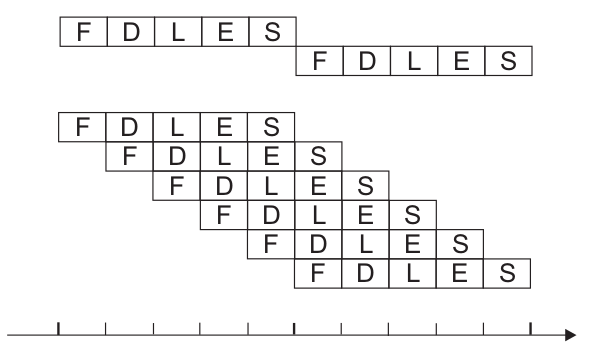
\includegraphics[scale=0.5]{images/pipeline.png}
\captionsource{Pipelined instruction processing in a five-stage pipeline.}{\cite[p. 45]{RTS}}
\label{pipeline}
\end{figure}
Der größte Nachteil an der seriellen Ausführung dieser Phasen besteht darin, dass zu jedem Zeitpunkt vier dieser fünf Elemente untätig ist. Wird beispielsweise gerade ein Befehl geladen, so sind sowohl Decoder, Datenbus als auch ALU untätig.\\
Somit wurde der Begriff der 'Pipeline' eingeführt, um dieses Problem zu umgehen. Hierbei werden zu jedem Zeitpunkt fünf Befehle zugleich verarbeitet, was in Abb. \ref{pipeline} sichtbar ist. Damit ergäbe sich eine Laufzeit von $(n+4) \cdot t$, da nach Beginn des letzten Befehls noch vier Zyklen vergehen, um diesen zu beenden.\\
Hier stellt sich jedoch die Frage, welcher Befehl als nächstes geladen wird. Beim seriellen Verfahren wird ein Ergebnis berechnet, gespeichert und auf dessen Grundlage der nächste Befehl gewählt. Bei einem parallelen Verfahren wird davon ausgegangen, dass die Befehle in sequentieller Form vorliegen und somit nach dem Befehl $n$ der Befehl $n+1$ benötigt wird. Solange dies zutrifft lässt sich eine Zeit von $(n+4) \cdot t$ einhalten. Wird jedoch ein 'falscher' Befehl geladen, so muss die Pipeline 'geflushed', also von allen Befehlen gereinigt werden. Dies erzeugt zusätzliche Laufzeit. Wird eine Pipeline in einem System angewendet, dessen Befehle nicht darauf angepasst worden sind und nicht in sequentieller Form vorliegen, so kann die Laufzeit die eines seriellen Systems übertreffen.\\
Somit lässt sich konkludieren, dass sich mithilfe von Pipelines massive Performance-Verbesserungen erzielen lassen, solange das System hierfür entsprechend angepasst wird.

\subsubsection{Multi-Core}
Die Taktfrequenz eines Prozessors ist nicht beliebig erhöhbar. Bei Frequenzen im geringen Gigahertz-Bereich sorgt die entstehende Abwärme dafür, dass sich die Hardware bereits nach kurzer Zeit selber zerstören würde. Ebenfalls wird die Synchronisation der Daten in solchen Frequenzbereichen kompliziert. Um die Leistungsfähigkeit eines Prozessors weiter erhöhen zu können sind Mehrkernprozessoren eingeführt worden. Jeder dieser Kerne besitzt einen eigenen 'Instuction\& Data-Cache', welche mit einem gemeinsamen 'Internal Cache Bus' verbunden sind. Dieser wiederum ist mit einem 'Common Instruction\& Data-Cache' verbunden, welcher die Schnittstelle zu dem 'System Bus' darstellt.\\
Theoretisch ist somit eine Vervielfachung des Durchsatzes an Aufgaben möglich, welche proportional zu der Anzahl an Kernen ist. Voraussetzung hierfür ist eine optimale Verteilung der Aufgaben auf die Kerne, sowie eine parallele Verarbeitung, Anforderung und Speicherung von Daten. Die Realisierung hiervon ist jedoch nicht trivial. Zudem führt ein Mehrkernprozessor gleichzeitig auch starken Nichtdeterminismus ein, welcher seinen Ursprung in der Verteilung der Aufgaben, Pipelines sowie den individuellen und dem gemeinsamen Cache findet. Des weiteren ist es wichtig, die Kommunikation zwischen den einzelnen Kernen zu gewährleisten, welche zuverlässig und, vor allem anderen, schnell möglich sein muss.\\
Bei gründlicher Planung und Gestaltung eines Mehrkernprozessors können enorme Fortschritte in der 'Geschwindigkeit' eines Prozessors erzielt werden, ohne sich um Hitzeentwicklung oder Gatterlaufzeiten Gedanken zu machen. Jedoch bieten sich auch weitaus mehr Aspekte, die anfällig für Fehler sind.

\subsection{CISC/RISC}\label{2.5}
Eine weitere notwendige Entscheidung bei der Gestaltung eines Systems wird von der Art der Befehlsatzes gestellt. Es gibt zwei vorherrschende Optionen - 'Complex Instruction Set Computers' (CISC) sowie 'Reduces Instruction Set Computers' (RISC). Diese unterscheiden sich in einer Vielzahl an Aspekten, beispielsweise die Anzahl der Befehle, deren Laufzeit und die Komplexität.

\subsubsection{Complex Instruction Set Computers}
Diese Art eines Befehlssatzes bietet eine Vielzahl komplexer Befehle, deren Ziele die Minimalisierung der Laufzeit, Reduktion des Speicherverbrauchs sowie vereinfachte Handhabung sind. Erreicht wird dies durch die Implementierung von frequentiert genutzten Anweisungen.\\
Als Beispiel diene folgender Befehl:\\

MULT $\$A, \$B$\\
\newline
Dieser Befehl sagt aus, dass die Werte der Register $A$ und $B$ geladen, multipliziert und in dem Register $A$ gespeichert werden. Dabei bezeichnet $\$A$ das Register mit der Nummer A. Die äquivalente Form eines 'RISC' sähe wie folgt aus:\\
\newpage
LOAD $x$, $\$A$\\ 
LOAD $y$, $\$B$\\
PROD $x$, $y$\\
STORE $\$A$, $x$\\
\newline
Hier werden die Register $A$ und $B$ in die Variablen $x$ und $y$ geladen, multipliziert, in der Variable $x$ zwischengespeichert und anschließend in dem Register $A$ gelagert. Es ist offensichtlich, dass die 'CISC'-Variante weitaus einfacher zu verwenden ist. Ebenfalls wird die Größe dieses Programms um 75\% reduziert, und somit werde weniger Daten von dem Hauptspeicher gelesen. Dies reduziert zusätzlich die Laufzeit des Codes.

\subsubsection{Reduces Instruction Set Computers}
Am vorangehenden Beispiel wird deutlich, dass sich 'RISC' auf elementare Befehle beschränkt. Der wohl wichtigste Aspekt ist, dass jeder Befehl genau einen Taktzyklus dauert. Durch diese einheitliche Laufzeit werden Pipelines und Parallelismus effizienter nutzbar. Der größte hierdurch entstehende Nutzen folgt daraus, dass ein Interrupt nach jedem Taktzyklus möglich ist. Ebenfalls ist somit kein Fokus auf bestimmte Befehle gelegt, sondern jede mögliche Kombination dieser elementaren Befehle ist denkbar. Ein weiterer Vorteil besteht in der reduzierten Speichernutzung dieser Befehle. Durch eine minimale Anzahl an sehr kompakten Befehlen wird nun ein Bruchteil des von einer 'CISC'-Variante genutzten Speichers benötigt.

\subsubsection{Anwendung bei einem DSP}
In der Regel wird ein 'DSP' mittels eines 'CISC' realisiert. Durch die schnelle Reaktion auf einen Interrupt sowie die geringe Anzahl an benötigten Befehlen eines 'DPS's bietet sich diese Wahl an. Die Implementierung von 'MAC'-Befehlen ist jedoch nicht optional und stellt den wichtigsten Aspekt dieses Systems dar. Der Begriff 'MAC' wird im folgenden behandelt.
\subsection{Scheduling}\label{2.6}
\subsection{System Service}\label{2.7}